\chapter{Results}

Every simulation is run ten times and the mean and standard deviation($\sigma$) is calculated. 

\section{Price}

\begin{figure}[!htb]
	\hspace*{-1cm}\ 
	\centering
	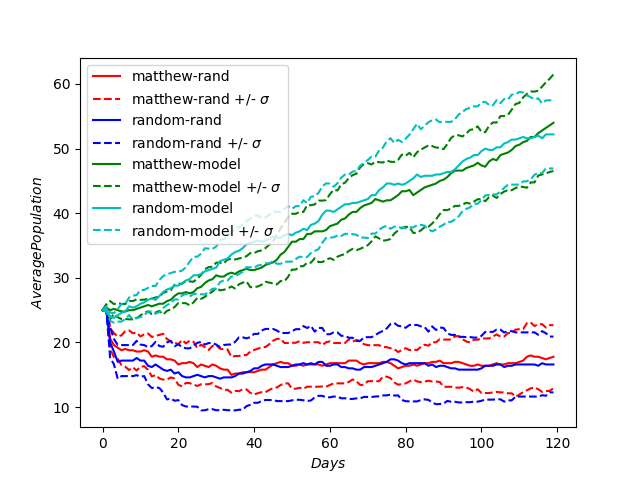
\includegraphics[width=9cm]{images/histories_deviation.png}
	\caption{ ...
	}
	\label{fig:fee_curve}
	\hspace*{2mm} 
\end{figure}

\begin{figure}[!htb]
	\hspace*{-1cm}\ 
	\centering
	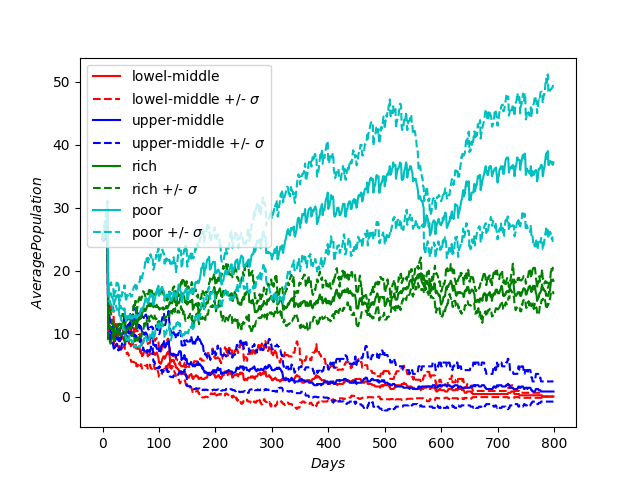
\includegraphics[width=9cm]{images/histories_deviation_fund.png}
	\caption{ ...
	}
	\label{fig:fee_curve}
	\hspace*{2mm} 
\end{figure}


(preferential attachment)

(pricing)

(funding)

(open close)

(degree distribution)
(profit distribution)

(re-balance channel)

(combined best strategies)

(is strategy set stable from invasion)

(external pressures, payment pressure, routing / private channels.)